\documentclass[11pt]{article}
\usepackage[margin=1in]{geometry}
\usepackage[utf8]{inputenc}
\usepackage{class-notes}

\title{Class Notes}
\author{}
\date{}

\begin{document}
\maketitle
\tableofcontents
\newpage

\section{Lecture 1}
\textit{Sep 24, 2025}

\subsection*{The two faces of quantum computation}

\begin{enumerate}
    \item[\textcircled{1}] The theoretical model of q. computation
    \begin{itemize}
        \item what we will explore in this class
        \item idealized, consistent, plausible description of reality
        \item ``implementation agnostic''
        \item testbed for algorithm design and proving impossibility results.
    \end{itemize}
    \item[\textcircled{2}] Implementations of q. computation
    \begin{itemize}
        \item Ion traps, photonic, Neutral atoms etc
        \item Models in which we hope to simulate idealized q.c.
        \item Not what we will explore but pertinent to q.c. implementations
    \end{itemize}
\end{enumerate}

\textbf{Lecture 1 plan:}
\begin{enumerate}
    \item[\textcircled{1}] Representation and manipulation of q. information
    \item[\textcircled{2}] An example of q. computing advantage.
\end{enumerate}

\subsection*{Notation}

We express vectors over $\mathbb{C}^d$ as follows:
\[
\ket{v} = \begin{pmatrix} v(0) \\ v(1) \\ \vdots \\ v(d-1) \end{pmatrix}
\qquad
\text{For } j \in \{0, \dots d-1\}
\qquad
\ket{j} = \begin{pmatrix} 0 \\ \vdots \\ 1 \\ \vdots \\ 0 \end{pmatrix}
\begin{matrix} \leftarrow 0^{\text{th}} \text{ pos.} \\ \\ \leftarrow j^{\text{th}} \text{ pos.} \\ \\ \leftarrow d-1^{\text{th}} \text{ pos.} \end{matrix}
\]

and because of its prevalence, we write
\[
\bra{v} = \begin{pmatrix} v(0)^* & v(1)^* & \dots & v(d)^* \end{pmatrix}
\]
\[
\uparrow \text{ complex conjugate.}
\]

Questions for class: (see pset 0 for length explanation).

\begin{enumerate}
    \item[\textcircled{1}] What is $\bra{v} \cdot \ket{v}$?

    we use short form $\braket{v}{v}$ for this.

    \item[\textcircled{2}] Let $M = \ket{w} \cdot \bra{v}$ (short form $\ket{w}\bra{v}$)

    for unit vectors $\ket{w}, \ket{v}$. What is $M\ket{v}$?
\end{enumerate}

\subsection*{Axioms of Q.C.}

\begin{quote}
\textbf{Axiom 1} [State description]

The state of exclusively one qubit can be expressed as a vector in $\mathbb{C}^2$ of unit norm.
\end{quote}

\[
\ket{\psi} = \begin{pmatrix} \alpha \\ \beta \end{pmatrix} \quad \text{s.t.} \quad |\alpha|^2 + |\beta|^2 = 1.
\]

\underline{Not:} Define $\ket{0} = \begin{pmatrix} 1 \\ 0 \end{pmatrix}$ and $\ket{1} = \begin{pmatrix} 0 \\ 1 \end{pmatrix}$

Note: $\ket{0} \neq 0$.

These form a orthonormal basis for $\mathbb{C}^2$ and are possible states for a qubit. If the state of a qubit is either $\ket{0}$ or $\ket{1}$, we call it ``classical''.

\underline{Ex.} $\dfrac{1}{\sqrt{2}}\left[\ket{0} + \ket{1}\right] = \dfrac{1}{\sqrt{2}}\left[\begin{pmatrix}1\\0\end{pmatrix} + \begin{pmatrix}0\\1\end{pmatrix}\right] = \dfrac{1}{\sqrt{2}}\begin{pmatrix}1\\1\end{pmatrix}$

is a non-classical --i.e. ``quantum''-- possible state.

\begin{quote}
\textbf{Axiom 2} Transformation of a qubit

Let $\mathcal{U}$ be a unitary matrix $\in \mathbb{C}^{2\times 2}$.

We can transform the state $\ket{\psi}$ to $\mathcal{U}\ket{\psi}$.
\end{quote}

\begin{figure}[h]
\centering
\begin{tikzpicture}[scale=1.1]
\fill[gray!20] (0,0) circle (2.6);
\draw (0,0) circle (2.6);
\draw[->] (-3,0) -- (3,0);
\draw[->] (0,-3) -- (0,3);
\node at (3.3,-0.3) {$\ket{0} = \binom{1}{0}$};
\node at (0.9,3.2) {$\ket{1} = \binom{1}{0}$};
\draw[->] (0,0) -- (60:2.6) coordinate (psi);
\node at (3.4,2.5) {$\ket{\psi} = \binom{\alpha}{\beta} \in \mathbb{C}^2$};
\draw[->] (0,0) -- (100:2.6) coordinate (Hpsi);
\node at (-0.6,3.0) {$H\ket{\psi}$};
\draw[->] (0,0) -- (25:2.6) coordinate (Xpsi);
\node at (3.3,1.1) {$X\ket{\psi}$};
\draw[->,blue] (0,0) -- (-60:2.6) coordinate (Zpsi);
\node[blue] at (1.9,-2.4) {$Z\ket{\psi}$};
\draw[blue,->] (psi) to[bend right=25] (Xpsi);
\draw[blue,->] (psi) to[bend left=15] (Zpsi);
\draw (0.5,0) arc (0:60:0.5);
\node at (0.45,0.22) {$\alpha$};
\end{tikzpicture}
\end{figure}

Recall $\mathcal{U}$ is a unitary iff (equivalently)
\begin{enumerate}
    \item[\textcircled{1}] $\mathcal{U}\ket{\psi}$ is unit iff $\ket{\psi}$ is unit.
    \item[\textcircled{2}] $\mathcal{U}^\dagger \mathcal{U} = \mathbb{1}$.
\end{enumerate}

\underline{Ex.} $X = \begin{pmatrix} 0 & 1 \\ 1 & 0 \end{pmatrix}$ \quad ``bit flip''

$Z = \begin{pmatrix} 1 & 0 \\ 0 & -1 \end{pmatrix}$ \quad ``phase flip''

$H = \dfrac{1}{\sqrt 2}\begin{pmatrix} 1 & 1 \\ 1 & -1 \end{pmatrix}$ \quad ``Hadamard''

\begin{quote}
\textbf{Axiom 3} (Measurement / Born's Rule)

Given a quantum state $\ket{\psi} = \begin{pmatrix}\alpha\\\beta\end{pmatrix}$, we can ``measure'' the quantum state meaning with

pr $|\braket{0}{\psi}|^2 = |\alpha|^2$, the state is now $\ket{0}$

pr $|\braket{1}{\psi}|^2 = |\beta|^2$, the state is now $\ket{1}$. \underline{\hspace{2cm}}\\
\hspace*{5cm}``collapses''

Plus, the classical value ``0'' or ``1'' is output.
\end{quote}

What does measuring twice in a row do?

If state is $\ket{0}$ or $\ket{1}$ measurement does not change the state.

Hence, why $\ket{0}$ or $\ket{1}$ are classical values

like classical objects, measurement/observations do not change the state.

\begin{figure}[h]
\centering
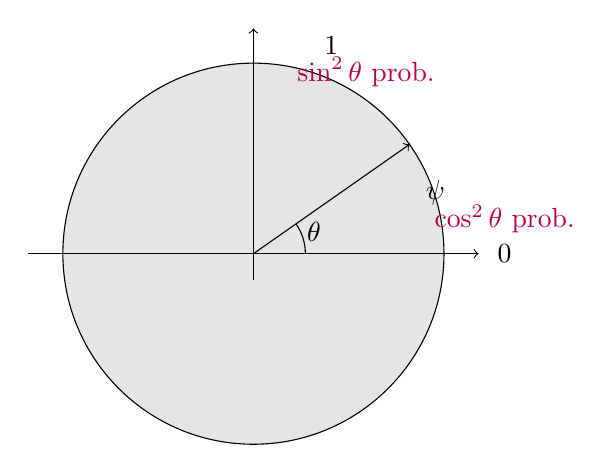
\begin{tikzpicture}[scale=1.1]
\fill[gray!20] (0,0) circle (2.2);
\draw (0,0) circle (2.2);
\draw[->] (-2.6,0) -- (2.6,0);
\draw[->] (0,-0.3) -- (0,2.6);
\draw[->] (0,0) -- (35:2.2) coordinate (psi2);
\node at (0.9,2.4) {$\ket{1}$};
\node[purple] at (1.3,2.1) {$\sin^2\theta$ prob.};
\node at (2.9,0) {$\ket{0}$};
\node at (2.1,0.7) {$\ket{\psi}$};
\node[purple] at (2.9,0.4) {$\cos^2\theta$ prob.};
\draw (0.6,0) arc (0:35:0.6);
\node at (0.7,0.25) {$\theta$};
\end{tikzpicture}
\end{figure}

\underline{Remark} $\theta \in [0,2\pi)$, the states $e^{i\theta}\ket{\psi}$ and $\ket{\psi}$ cannot be distinguished by measurement.

\underline{Pf:} $\Pr[e^{i\theta}\ket{\psi} \text{ collapsing to } j]$
\begin{align*}
&= |\bra{j} e^{i\theta} \ket{\psi}|^2 \\
&= \bra{\psi} e^{-i\theta} \ket{j} \braket{j}{e^{i\theta}\psi} \\
&= e^{-i\theta} e^{i\theta} \braket{\psi}{j}\braket{j}{\psi} \\
&= \Pr[\ket{\psi} \text{ collapsing to } j].
\end{align*}

$e^{i\theta}$ is defined as the ``global phase''.

Quantum states form an equivalence class for $\ket{\psi} \sim e^{i\theta}\ket{\psi}$ and set of states is $\mathbb{C}^2/{\sim}$.

\begin{quote}
\textbf{Axiom 4} (Initialization)

We can initialize a qubit as $\ket{0}$.
\end{quote}

These axioms already imply a perfect random number generator.
\begin{enumerate}
    \item[\textcircled{1}] Initialize qubit as $\ket{\psi_0} = \ket{0} = \begin{pmatrix}1\\0\end{pmatrix}$.
    \item[\textcircled{2}] Apply $H$ transform:
    \[
    \ket{\psi_1} = H\ket{\psi_0} = \frac{1}{\sqrt2}\begin{pmatrix}1&1\\1&-1\end{pmatrix}\begin{pmatrix}1\\0\end{pmatrix} = \begin{pmatrix} 1/\sqrt2 \\ 1/\sqrt2 \end{pmatrix}.
    \]
    \item[\textcircled{3}] Measure the qubit.

    w pr $|\bra{0}\psi_1\rangle|^2 = \left|\dfrac{1}{\sqrt2}\right|^2 = \dfrac12$ collapses to $\ket{0}$.

    w pr $|\bra{1}\psi_1\rangle|^2 = \left|\dfrac{1}{\sqrt2}\right|^2 = \dfrac12$ collapses to $\ket{1}$.
\end{enumerate}

\subsection*{Multiple qubits}

Recall the notion of tensor products

\[
A \in \mathbb{C}^{m_1 \times n_1}, \qquad B \in \mathbb{C}^{m_2 \times n_2}
\]
\[
A = \begin{pmatrix} A_{11} & A_{12} & \dots & A_{1n_1} \\ A_{21} & A_{22} & & A_{2n_1} \\ \vdots & & \ddots & \\ A_{m_1 1} & & & A_{m_1 n_1} \end{pmatrix}, \qquad
B = \begin{pmatrix} B_{11} & \dots & B_{1n_2} \\ \vdots & & \vdots \\ B_{m_2 1} & & B_{m_2 n_2} \end{pmatrix}
\]

$A \otimes B \in \mathbb{C}^{m_1 m_2 \times n_1 n_2}$

\[
A \otimes B = \begin{pmatrix} A_{11}\cdot B & A_{12}\cdot B & \dots & A_{1n_1}\cdot B \\ \vdots & & \ddots & \\ A_{m_1 1}\cdot B & & & A_{m_1 n_1}\cdot B \end{pmatrix}
\]
i.e. each block $A_{ij}\cdot B$ is itself the $m_2 \times n_2$ block $\begin{pmatrix} A_{ij}B_{11} & \dots & A_{ij}B_{1n_2} \\ \vdots & & \vdots \\ A_{ij}B_{m_2 1} & \dots & A_{ij}B_{m_2 n_2} \end{pmatrix}$, arranged in the full $m_1\times n_1$ grid of blocks.

\underline{Properties of the tensor product (hw 1):}

$A \in \mathbb{C}^{\ell_1\times m_1}$ \quad $B \in \mathbb{C}^{\ell_2\times m_2}$ \hfill note: vectors are matrices too!

$C \in \mathbb{C}^{m_1\times n_1}$ \quad $D \in \mathbb{C}^{m_2\times n_2}$

so $AC \in \mathbb{C}^{\ell_1\times n_1}$ \quad $BD \in \mathbb{C}^{\ell_2\times n_2}$

\begin{enumerate}
    \item[\textcircled{1}] $(A\otimes B)(C\otimes D) = AC \otimes BD$.
    \item[\textcircled{2}] linearity. ex. $(A\otimes B)\left(\sum_i C_i \otimes D_i\right) = \sum_i AC_i \otimes BD_i$.
    \item[\textcircled{2}] $(A\otimes B)^\dagger = A^\dagger \otimes B^\dagger$
    \item[\textcircled{3}] $(A\otimes B)^{-1} = A^{-1}\otimes B^{-1}$ when invertible.
\end{enumerate}

We can also take tensor products of vectors as vectors are 1-D matrices.

\underline{Exercises}
\begin{enumerate}
    \item[\textcircled{1}] What is $\ket{0}\otimes\ket{1}\otimes\ket{0}$?
    \item[\textcircled{2}] What is $\ket{0}\otimes\ket{1}\otimes\ket{1}$?
\end{enumerate}

\underline{Notation} $\ket{0}\otimes\ket{1}\otimes\ket{0} = \ket{0}\ket{1}\ket{0} = \ket{0,1,0}$

\underline{Remark} $\ket{x_1,x_2,\dots,x_n}$ for $x_i \in \{0,1\}$ is the $x^{\text{th}}$ basis vector when $x = x_1\dots x_n$ is interpreted in binary.

Better notation: $\ket{0}\otimes\ket{1}\otimes\ket{0} = \ket{010}$

So for $j \in \{0,\dots,2^n-1\}$ we write
\[
\ket{j} = \ket{j_1 j_2 \dots j_n} = \ket{j_1}\otimes\dots\otimes\ket{j_n}
\]
where $j_1\dots j_n$ is binary value of $j$. \hfill Note: orthogonality.

Additionally, when considering vectors in $\mathbb{C}^d$, we use
\[
\ket{j} = \begin{pmatrix} 0 \\ 0 \\ \vdots \\ 1 \\ \vdots \\ 0 \end{pmatrix}
\begin{matrix} \leftarrow 0^{\text{th}} \text{location} \\ \\ \\ \leftarrow j^{\text{th}} \text{location} \\ \\ \leftarrow d-1^{\text{th}} \text{location} \end{matrix}
\qquad \text{for } j \in \{0,\dots d-1\}
\]

This matches the binary description of the vector.

\subsection*{Bringing multiple qubits together}

If we have qubit $A$ in state $\ket{\psi_A}$ and qubit $B$ in state $\ket{\psi_B}$,

We need a way to describe the state of the 2 qubits.

\[
\ket{\Psi}_{AB} = \ket{\psi}_A \otimes \ket{\varphi}_B.
\]

We need axioms to describe the composite system
\begin{enumerate}
    \item[\textcircled{1}] If qubits don't interact, should reproduce statistics of 1 qubit.
    \item[\textcircled{2}] A method for entangling the qubits.

    i.e. for any vector $\ket{\psi} \in (\mathbb{C}^2)^{\otimes 2}$

    there exists a method of generating said state.
\end{enumerate}

\underline{Updated Axioms for $n$ qubits:}
\begin{enumerate}
    \item[\textcircled{1}] The state of a $n$ qubit system is a unit vec in
    \[
    \underbrace{\mathbb{C}^2 \otimes \mathbb{C}^2 \otimes \dots \otimes \mathbb{C}^2}_{n \text{ times}} = (\mathbb{C}^2)^{\otimes n} \cong \mathbb{C}^{2^n} =: \mathcal{H} \quad \text{Hilbert space.}
    \]
\end{enumerate}

Every quantum state $\ket{\psi} \in (\mathbb{C}^2)^{\otimes n}$ is a unit vec.

\[
\begin{pmatrix} \psi(0\dots0) \\ \psi(0\dots1) \\ \psi(0\dots10) \\ \vdots \\ \psi(1\dots1) \end{pmatrix}
=
\begin{pmatrix} \psi(0) \\ \psi(1) \\ \vdots \\ \vdots \\ \psi(2^n-1) \end{pmatrix}
\]

\[
\ket{\psi} = \sum_{x=0}^{2^n-1} \psi(x_1x_2\dots x_n)\ket{x_1,\dots,x_n} = \sum_x \underbrace{\psi(x)}_{\text{amplitude}}\ket{x}
\]

$\ket{\psi}$ is classical if all amplitudes are 0 except 1.

$\ket{\psi}$ is in superposition if there are multiple non-zero amplitudes.

\begin{enumerate}
    \item[\textcircled{2}] For any unitary $\mathcal{U} \in \mathbb{C}^{4\times4}$, we can transform the state $\ket{\psi}$ to
    \[
    \Big[\underbrace{\mathbb{1}_2 \otimes \dots \otimes \mathbb{1}_2}_{\ell_1} \otimes \mathcal{U} \otimes \underbrace{\mathbb{1}_2\otimes\dots\otimes\mathbb{1}_2}_{\ell_2}\Big]\ket{\psi}, \qquad \ell_1 + 2 + \ell_2 = n
    \]
\end{enumerate}

this only allows action between adjacent qubits but this turns out to be sufficient (hw 1).

Then,
\[
\left(\mathbb{1}_2\otimes\dots\otimes\mathbb{1}_2\otimes\mathcal{U}\otimes\mathbb{1}_2\dots\otimes\mathbb{1}_2\right)\ket{x_1\dots x_n}
\]
\[
= \Big(\ket{x_1}\ket{x_2}\dots\ket{x_{i-1}}\Big) \otimes \mathcal{U}\ket{x_i,x_{i+1}} \otimes \Big(\ket{x_{i+2}}\dots\ket{x_n}\Big)
\]
\[
= \Big(\ket{x_1}\ket{x_2}\dots\ket{x_{i-1}}\Big) \otimes \sum_{k_1,k_2} \mathcal{U}_{(k_1k_2)(x_i,x_{i+1})}\ket{k_1,k_2} \otimes \Big(\ket{x_{i+2}}\dots\ket{x_n}\Big)
\]

By linearity we can compute
\[
\left(\mathbb{1}_2\otimes\dots\otimes\mathbb{1}_2\otimes\mathcal{U}\otimes\mathbb{1}_2\dots\otimes\mathbb{1}_2\right)\ket{\psi}
\]
for any $\ket{\psi}\in(\mathbb{C}^2)^{\otimes n}$ by expressing
\[
\ket{\psi} = \sum_{x_1\dots x_n} \underbrace{\psi(x_1\dots x_n)}_{\text{amplitude}}\ket{x_1,\dots,x_n}
\]

A unitary $\mathcal{U} \in \mathbb{C}^{2^k \times 2^k}$ is also called a $k$-qubit unitary. In particular, $\mathcal{U}\in\mathbb{C}^{2\times2}$ is a single-qubit unitary and $\mathcal{U}\in\mathbb{C}^{4\times4}$ is a 2-qubit unitary.

\[
\underbrace{\mathbb{1}_2\otimes\dots\otimes\mathbb{1}_2}_{\substack{\uparrow\\\text{acting on}\\\text{qubit }1}} \otimes \underbrace{\mathcal{U}}_{\substack{\uparrow\\\text{acting on}\\\text{qubits }i \,\&\, i{+}1}} \otimes \underbrace{\mathbb{1}_2\dots\otimes\mathbb{1}_2}_{\substack{\uparrow\\\text{acting on}\\\text{qubit }n}}
\]

is a general q.c. unitary transform.

say $\mathcal{U} = \begin{pmatrix} \mathcal{U}_{(0,0),(0,0)} & \mathcal{U}_{(0,0),(0,1)} & \dots & \mathcal{U}_{(0,0),(1,1)} \\ \vdots & & & \\ \mathcal{U}_{(1,1),(0,0)} & \dots & & \mathcal{U}_{(1,1),(1,1)} \end{pmatrix}$

i.e. $\displaystyle \mathcal{U} = \sum_{k_1k_2j_1j_2 \in \{0,1\}} \mathcal{U}_{(k_1,k_2)(j_1,j_2)} \ket{k_1,k_2}\bra{j_1,j_2}$

\begin{enumerate}
    \item[\textcircled{3}] Measurement of all qubits. ($n$-qubit Born's rule)

    For $j \in \{0,\dots 2^n-1\}$,

    w pr $|\braket{j}{\psi}|^2$ collapse to $\ket{j}$ and output ``$j$''.
\end{enumerate}

Problem set 1 will introduce how to measure arbitrary single qubits.

\begin{enumerate}
    \item[\textcircled{3}$'$] measurement of the $1^{st}$ qubit.

    $\ket{\psi} = \ket{0}\otimes\ket{\psi_0} + \ket{1}\otimes\ket{\psi_1}$. \hfill $\ket{\psi} = \begin{pmatrix}\ket{\psi_0}\\\ket{\psi_1}\end{pmatrix}$

    w pr $\|\ket{\psi_0}\|^2$ collapse to $\ket{0}\otimes\dfrac{\ket{\psi_0}}{\|\ket{\psi_0}\|}$.

    w pr $\|\ket{\psi_1}\|^2$ collapse to $\ket{1}\otimes\dfrac{\ket{\psi_1}}{\|\ket{\psi_1}\|}$.
\end{enumerate}

\begin{enumerate}
    \item[\textcircled{4}] Given $n$-qubit state $\ket{\psi}$, we can initialize a ``fresh'' qubit as $\ket{0}$, generating state $\ket{\psi}\otimes\ket{0}$ (unentangled) on $(n+1)$-qubits.
\end{enumerate}

More generally, we can join q. systems $\ket{\psi}_A \otimes \ket{\psi_B}$ from $\ket{\psi_A}$ and $\ket{\psi_B}$.

And we can separate unentangled systems.

\textcolor{blue}{These are not axioms as we can derive them from the axioms.}

Why does this def satisfy uninteracting qubit statistics.

\[
\ket{\Psi} = \ket{\psi}\otimes\ket{\varphi}
\]
\[
\hspace{2cm}\underbrace{\hspace{1.2cm}}_{1\text{ qubit}}\underbrace{\hspace{2cm}}_{\text{multiple qubits}}
\]

If $\ket{\psi} = \alpha\ket0 + \beta\ket1$.

Then
\[
\ket{\Psi} = \alpha\ket{0}\ket{\varphi} + \beta\ket{1}\ket{\varphi} = \ket{0}\alpha\ket{\varphi} + \ket{1}\beta\ket{\varphi}.
\]

So, pr $\|\alpha\ket{\varphi}\|^2 = |\alpha|^2$ collapses to $\dfrac{\alpha\ket{\varphi}}{|\alpha|}$

pr $|\beta|^2$ collapses to $\dfrac{\beta\ket{\varphi}}{|\beta|}$.

So remaining state remains $\propto \ket{\varphi}$.

Matches our intuition for what should happen.

\subsection*{Important math review: Prob. Theory}

Let $X\geq 0$ be a pos. random variable.
\begin{enumerate}
\item[\textcircled{1}]
\underline{Markov's Ineq.} $\Pr[X\geq a] \leq \dfrac{\mathbb{E}X}{a}$ for all $a>0$.

\underline{Pf.} $\mathbb{E}X = \underbrace{\mathbb{E}[X\mid X\geq a]}_{\geq a}\cdot\Pr[X\geq a] + \underbrace{\mathbb{E}[X\mid X<a]}_{0}\underbrace{\Pr[X<a]}_{0}$
\end{enumerate}

\begin{enumerate}
\setcounter{enumi}{1}
\item[\textcircled{2}]
Let $X$ be a r.v. with $\mathrm{Var}\,X = \sigma^2$ finite and $\mathbb{E}X = \mu$.

\underline{Chebyshev's Ineq.} $\forall k>0$,
\[
\Pr[\,|X-\mu|\geq k\sigma\,] \leq \frac{1}{k^2}.
\]

\underline{Pf.} Apply Markov for $Y = (X-\mu)^2$ and $a = k^2\sigma^2$.
\[
\Pr[|X-\mu|\geq k\sigma] = \Pr[(X-\mu)^2 \geq k^2\sigma^2] = \Pr[Y\geq k^2\sigma^2] \leq \frac{\mathbb{E}Y}{k^2\sigma^2} = \frac{\sigma^2}{k^2\sigma^2} = \frac{1}{k^2}.
\]
\end{enumerate}

\begin{enumerate}
\setcounter{enumi}{2}
\item[\textcircled{3}] Chernoff bounds:
\[
\Pr[X\geq a] = \Pr[e^{tX}\geq e^{ta}] \leq \frac{\mathbb{E}[e^{tX}]}{e^{ta}} \quad \text{(Markov's)}
\]
So, $\displaystyle \Pr[X\geq a] \leq \inf_{t>0} \frac{\mathbb{E}[e^{tX}]}{e^{ta}}$.

If $X = X_1+\dots+X_n$, then
\[
\Pr[X\geq a] = \inf_{t>0} e^{-ta}\prod_{i=1}^n \mathbb{E}[e^{tX_i}].
\]
\end{enumerate}

If $X_i \in \{0,1\}$ then $e^{tX_i} = \begin{cases} e^t & \text{pr } p_i := \mathbb{E}X_i \\ 1 & \text{pr } 1-p_i \end{cases}$

\[
\mathbb{E}e^{tX_i} = (e^t-1)p_i + 1 \leq e^{p_i(e^t-1)}.
\]

So, $\displaystyle\prod_i \mathbb{E}e^{tX_i} \leq e^{(p_1+\dots+p_n)(e^t-1)} = e^{\mu(e^t-1)}$, \quad $\mu = \mathbb{E}X = p_1+\dots+p_n$.

Let $a = (1+\delta)\mu$.
\[
\inf_{t>0} e^{-ta}\prod_i \mathbb{E}[e^{tX_i}] \leq \inf_{t>0} e^{-t(1+\delta)\mu} e^{\mu(e^t-1)} \leq \inf_{t\geq0}\left(e^{\left(\frac{e^t-1}{(1+\delta)t}\right)}\right)^\mu
\]
\[
= \left(\frac{e^\delta}{(1+\delta)^{1+\delta}}\right)^\mu \leq e^{-\delta^2\mu/(2+\delta)}. \qquad \text{\underline{Ex.} inf at } t=\ln(1+\delta). \text{ (exercise)}
\]

\underline{Chernoff bounds:} $X_1,\dots,X_n\in\{0,1\}$, $X=\sum X_i$, $\mu=\mathbb{E}X$.
\[
\Pr[X\geq(1+\delta)\mu] \leq e^{-\delta^2\mu/(2+\delta)}
\]
\[
\Pr[X\leq(1-\delta)\mu] \leq e^{-\delta^2\mu/2}
\]
\[
\Pr[\,|X-\mu|\geq\delta\mu\,] \leq 2e^{-\delta^2\mu/3}
\]

\section{Lecture 2}
\textit{Sep 29, 2025}

\subsection*{Important math review: Prob. Theory}

Let $X\geq 0$ be a pos. random variable.
\begin{enumerate}
\item[\textcircled{1}]
\underline{Markov's Ineq.} $\Pr[X\geq a] \leq \dfrac{\mathbb{E}X}{a}$ for all $a>0$.

\underline{Pf.} $\mathbb{E}X = \underbrace{\mathbb{E}[X\mid X\geq a]}_{\geq a}\cdot\Pr[X\geq a] + \underbrace{\mathbb{E}[X\mid X<a]}_{0}\underbrace{\Pr[X<a]}_{0}$
\end{enumerate}

\begin{enumerate}
\setcounter{enumi}{1}
\item[\textcircled{2}]
Let $X$ be a r.v. with $\mathrm{Var}\,X = \sigma^2$ finite and $\mathbb{E}X = \mu$.

\underline{Chebyshev's Ineq.} $\forall k>0$,
\[
\Pr[\,|X-\mu|\geq k\sigma\,] \leq \frac{1}{k^2}.
\]

\underline{Pf.} Apply Markov for $Y = (X-\mu)^2$ and $a = k^2\sigma^2$.
\[
\Pr[|X-\mu|\geq k\sigma] = \Pr[(X-\mu)^2 \geq k^2\sigma^2] = \Pr[Y\geq k^2\sigma^2] \leq \frac{\mathbb{E}Y}{k^2\sigma^2} = \frac{\sigma^2}{k^2\sigma^2} = \frac{1}{k^2}.
\]
\end{enumerate}

\begin{enumerate}
\setcounter{enumi}{2}
\item[\textcircled{3}] Chernoff bounds:
\[
\Pr[X\geq a] = \Pr[e^{tX}\geq e^{ta}] \leq \frac{\mathbb{E}[e^{tX}]}{e^{ta}} \quad \text{(Markov's)}
\]
So, $\displaystyle \Pr[X\geq a] \leq \inf_{t>0} \frac{\mathbb{E}[e^{tX}]}{e^{ta}}$.

If $X = X_1+\dots+X_n$, then
\[
\Pr[X\geq a] = \inf_{t>0} e^{-ta}\prod_{i=1}^n \mathbb{E}[e^{tX_i}].
\]
\end{enumerate}

If $X_i \in \{0,1\}$ then $e^{tX_i} = \begin{cases} e^t & \text{pr } p_i := \mathbb{E}X_i \\ 1 & \text{pr } 1-p_i \end{cases}$

\[
\mathbb{E}e^{tX_i} = (e^t-1)p_i + 1 \leq e^{p_i(e^t-1)}.
\]

So, $\displaystyle\prod_i \mathbb{E}e^{tX_i} \leq e^{(p_1+\dots+p_n)(e^t-1)} = e^{\mu(e^t-1)}$, \quad $\mu = \mathbb{E}X = p_1+\dots+p_n$.

Let $a = (1+\delta)\mu$.
\[
\inf_{t>0} e^{-ta}\prod_i \mathbb{E}[e^{tX_i}] \leq \inf_{t>0} e^{-t(1+\delta)\mu} e^{\mu(e^t-1)} \leq \inf_{t\geq0}\left(e^{\left(\frac{e^t-1}{(1+\delta)t}\right)}\right)^\mu
\]
\[
= \left(\frac{e^\delta}{(1+\delta)^{1+\delta}}\right)^\mu \leq e^{-\delta^2\mu/(2+\delta)}. \qquad \text{\underline{Ex.} inf at } t=\ln(1+\delta). \text{ (exercise)}
\]

\underline{Chernoff bounds:} $X_1,\dots,X_n\in\{0,1\}$, $X=\sum X_i$, $\mu=\mathbb{E}X$.
\[
\Pr[X\geq(1+\delta)\mu] \leq e^{-\delta^2\mu/(2+\delta)}
\]
\[
\Pr[X\leq(1-\delta)\mu] \leq e^{-\delta^2\mu/2}
\]
\[
\Pr[\,|X-\mu|\geq\delta\mu\,] \leq 2e^{-\delta^2\mu/3}
\]

Today: Quantum's power over classical
\begin{enumerate}
    \item[\textcircled{1}] Elitzar-Vaidman Bomb Tester
    \item[\textcircled{2}] Deutsch-Jozsa game.
\end{enumerate}

Recall axioms of quantum computation:
\begin{enumerate}
    \item[\textcircled{1}] The state of a $n$ qubit system is a unit vec in
    \[
    \underbrace{\mathbb{C}^2 \otimes \mathbb{C}^2 \otimes \dots \otimes \mathbb{C}^2}_{n \text{ times}} = (\mathbb{C}^2)^{\otimes n} \cong \mathbb{C}^{2^n}
    \]
    \item[\textcircled{2}] For any unitary $\mathcal{U} \in \mathbb{C}^{4\times4}$, we can transform the state $\ket{\psi}$ to
    \[
    \Big[\underbrace{\mathbb{1}_2 \otimes \dots \otimes \mathbb{1}_2}_{\ell_1} \otimes \mathcal{U} \otimes \underbrace{\mathbb{1}_2\otimes\dots\otimes\mathbb{1}_2}_{\ell_2}\Big]\ket{\psi}, \qquad \ell_1 + 2 + \ell_2 = n
    \]
    \item[\textcircled{3}] Measure the first qubit: $\ket{\psi} = \ket{0}\ket{\psi_0} + \ket{1}\ket{\psi_1}$

    Transform to $\dfrac{\ket{i}\ket{\psi_i}}{\|\ket{\psi_i}\|}$ with pr $\|\ket{\psi_i}\|^2$.

    \item[\textcircled{4}] Given state $\ket{\psi}$ on $n$-qubits, we can generate the state $\ket{\psi}\otimes\ket{0}$ on $(n+1)$-qubits
\end{enumerate}

\underline{Obs} General basis single-qubit measurements.

Let $\ket{b_0},\ket{b_1}$ be orthonormal vectors in $\mathbb{C}^2$.

Axioms give us a way to measure $\ket{\psi}$ and get

$\ket{0}$ w pr $|\bra{0}\psi\rangle|^2$ and

$\ket{1}$ w pr $|\bra{1}\psi\rangle|^2$.

Can we generate a method to get

$\ket{b_0}$ w pr $|\braket{b_0}{\psi}|^2$ and

$\ket{b_1}$ w pr $|\braket{b_1}{\psi}|^2$.

\underline{Ans} let $\mathcal{U} = \begin{pmatrix} | & | \\ \ket{b_0} & \ket{b_1} \\ | & | \end{pmatrix}$

$\mathcal{U}$ is unitary as $\mathcal{U}^\dagger = \begin{pmatrix} -\bra{b_0}- \\ -\bra{b_1}- \end{pmatrix}$

Then $\mathcal{U}^\dagger\mathcal{U} = \begin{pmatrix} \braket{b_0}{b_0} & \braket{b_0}{b_1} \\ \braket{b_1}{b_0} & \braket{b_1}{b_1} \end{pmatrix} = \begin{pmatrix}1&0\\0&1\end{pmatrix} = \mathbb{1}_2$.

For $i \in \{0,1\}$, $\mathcal{U}\ket{i} = \ket{b_i}$ so $\mathcal{U}^\dagger\ket{b_i} = \ket{i}$.

\underline{Algorithm}
\begin{enumerate}
    \item[\textcircled{1}] Apply $\mathcal{U}^\dagger$ (also unitary)
    \item[\textcircled{2}] Measure
    \item[\textcircled{3}] Apply $\mathcal{U}$.
\end{enumerate}

\underline{Pf.} state after \textcircled{1} is $\mathcal{U}^\dagger\ket{\psi}$

For $i \in \{0,1\}$, measuring produces $\ket{i}$ with pr
\[
|\bra{i}\mathcal{U}^\dagger\ket{\psi}|^2 = |\braket{b_i}{\psi}|^2
\]
Then applying $\mathcal{U}$ means we produce $\mathcal{U}\ket{i} = \ket{b_i}$ w pr $|\braket{b_i}{\psi}|^2$.

\subsection*{A physics motivation for qubits.}

Polarization of light.

Photons have a polarization:

Photons that travel $\leftrightarrow$ \quad ``in state'' $\ket{0}$

Photons that travel $\updownarrow$ \quad ``in state'' $\ket{1}$

Photons that travel $\nearrow$ \quad ``in state'' $\dfrac{\ket{0}+\ket{1}}{\sqrt2} =: \ket{+}$.

Build a sieve: 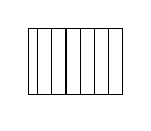
\begin{tikzpicture}[baseline=-0.3em,scale=0.6] \draw (0,0) rectangle (2,1.4); \foreach \x in {0.2,0.5,...,1.9} \draw (\x,0) -- (\x,1.4); \end{tikzpicture} \quad so that

output photons are polarized as $\ket{1}$. \quad
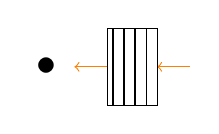
\begin{tikzpicture}[scale=0.7]
\draw[orange,->] (2.2,0.7) -- (1.6,0.7);
\draw (0.7,0) rectangle (1.6,1.4);
\foreach \x in {0.8,1.0,...,1.5} \draw (\x,0) -- (\x,1.4);
\draw[orange,->] (0.7,0.7) -- (0.1,0.7);
\node at (-0.4,0.7) {\Large $\bullet$};
\end{tikzpicture}

What is happening as photon hits the sieve?

\underline{Ans} measurement:
\[
\ket{\psi} = \alpha\ket0+\beta\ket1 = \begin{pmatrix}\alpha\\\beta\end{pmatrix} \quad \text{state of photon before.}
\]
collapses to either $\ket0$ ``absorbed'' w pr $|\alpha|^2$

\hspace{2.7cm} $\ket1$ ``goes through'' w pr $|\beta|^2$.

Random light's polarization can be thought of as a random angle. Easy to show that $\sim 1/2$ of photons pass through in the stat. mech. limit.

\underline{Problems:}

\emph{(diagram: a sieve at $90^\circ$ (vertical lines) lets no light through; a sieve at $0^\circ$ (horizontal lines) placed in front of a light source lets light through.)}

\emph{(diagram: a sieve at $45^\circ$ placed after a sieve at $0^\circ$ in front of a light source -- this is a non-standard basis measurement, and the light intensity should dim by about half.)}

Another way to analyze this is to notice that a sieve at angle $\theta$ is measuring the qubit in a non-standard basis given by

\[
\ket{b_0^\theta} = \cos\theta\ket0 + \sin\theta\ket1 \quad \text{``pass through''}
\]
\[
\ket{b_1^\theta} = -\sin\theta\ket0 + \cos\theta\ket1. \quad \text{``absorb''}.
\]

\emph{(diagram: light source, then a sieve at angle $\gamma$, then a sieve at angle $\gamma+\theta$.)}

What fraction of light passes through?

\[
\Pr\Big[\boxed{\ket{\gamma}_{\theta+\gamma} \text{ measurement accepts } \ket{b_0^\gamma}}\Big]
\]
\[
= |\braket{b_0^{\theta+\gamma}}{b_0^\gamma}|^2
\]
\[
= \big(\cos\gamma\cos(\theta+\gamma) + \sin\gamma\sin(\theta+\gamma)\big)^2
\]
\[
= \cos^2\big((\theta+\gamma)-\gamma\big) = \boxed{\cos^2\theta}.
\]

\subsection*{Elitzur-Vaidman Bomb Tester (1993)}

Suppose there is a black box (cannot open/see components) s.t.
\begin{enumerate}
    \item[(a)] A photon enters and a photon leaves.
    \item[(b)] you know it is 1 of 2 possibilities:
\end{enumerate}

``Bomb'' \quad \emph{(diagram: a box containing a sieve and a bomb symbol.)} If sieve measurement yields $\ket1$, bomb explodes. Otherwise photon passes through.

``Dud'' \quad \emph{(diagram: an empty box that a photon passes straight through.)}

Question: Can we detect which box is in front of us without setting off the bomb?

\underline{Ideas:}

send $\ket{\psi_{in}} = \ket0$

Dud: $\ket{\psi_{out}} = \ket0$. \hfill \underline{no difference.}

Bomb: $\ket{\psi_{out}} = \ket0$.

send $\ket{\psi_{in}} = \ket1$

Dud: $\ket{\psi_{out}} = \ket1$.

Bomb: \{Explosion\} \hfill \underline{too much difference.}

Model the Dud as the identity transform

the Bomb as a standard basis measurement.

Let's send in a rotated state

and measure the output in a rotated basis.

Introduce a rotational gate:

$R_\theta\ket\psi \longleftarrow$ \emph{(circle/lens symbol labeled $\theta$)} $\longleftarrow \ket\psi$

\[
R_\theta = \begin{pmatrix} \cos\theta & -\sin\theta \\ \sin\theta & \cos\theta \end{pmatrix}. \qquad
\begin{aligned} R_\theta\ket0 &= \cos\theta\ket0 + \sin\theta\ket1 \\ R_\theta^\dagger &= R_{-\theta}. \end{aligned}
\]

Diagram: \emph{(a rotated sieve at angle $\theta_2$, a ``?'' black box, and a lens $\theta_1$ acting on $\ket0$, in a row; measure if passes or reflects.)}

\underline{Quantum circuit:} (read right to left, state $\ket0$ enters on the right)
\[
\ket0 \;\to\; R_{\theta_1} \;\to\; \fbox{?} \;\to\; \fbox{$R_{\theta_1}$} \;\to\; \underbrace{\fbox{$\times$}}_{\theta_2 \text{ basis measurement}}
\]

by prev. we can write it as
\[
\ket0 \;\to\; R_{\theta_1} \;\to\; \fbox{?} \;\to\; R_{\theta_2}^\dagger \;\to\; \underbrace{\fbox{$\times$}}_{\text{standard}} \;\to\; R_{\theta_2} \qquad \text{\textcolor{blue}{irrelevant}}
\]

\[
R_{\theta_2}^\dagger = R_{-\theta_2} = R_{\theta_1-\theta_2}R_{-\theta_1}
\]

\[
\ket0 \;\to\; R_{\theta_1} \;\to\; \fbox{?} \;\to\; R_{-\theta_1} \;\to\; R_{\theta_1-\theta_2} \;\to\; \fbox{$\times$}
\]

when $\fbox{?} = \fbox{$\mathbb{1}$}$ ``dud''

this simplifies to $\ket0 \;\to\; R_{\theta_1-\theta_2} \;\to\; \fbox{$\times$}$

which ``accepts'' w pr $\cos^2(\theta_1-\theta_2)$, (no explosion)

``rejects'' w pr $\sin^2(\theta_1-\theta_2)$. (no explosion)

when $\fbox{?} = \fbox{$\times$}$ ``bomb''

$\ket0 \;\to\; R_{\theta_1} \;\to\; \fbox{$\times$} \;\to\; R_{\theta_1-\theta_2} \;\to\; \fbox{$\times$}$

``explode'' w pr $\sin^2(-\theta_1) = \sin^2(\theta_1)$.

``survive'' w pr $\cos^2(\theta_1)$.

\[
\Pr[\text{``accept''} \mid \text{``survive''}] = \cos^2(\theta_2).
\]
\[
\Pr[\text{``reject''} \mid \text{``survive''}] = \sin^2(\theta_2).
\]

say we are willing to tolerate $\epsilon$ prob. of explosion.

Want to pick $\theta_1$ s.t. $\epsilon = \sin^2(\theta_1)$.

what $\theta_2$ should we pick?

Equivalent to comparing two biased coins.

Coin$_{dud}$ tails with prob. $\sin^2(\theta_1-\theta_2)$

Coin$_{bomb}$ tails with prob. $\sin^2(\theta_2)$.

Pset 2 will discuss optimal distinguishing measurements.

For now, notice $\theta_2 = \theta_1$ yields that ``dud'' always accepts

and ``bomb'': explodes w pr $\epsilon$,

\hspace{2.3cm} rejects w pr $\epsilon(1-\epsilon)\approx\epsilon$

\hspace{2.3cm} accepts w pr $(1-\epsilon)^2 \approx 1-2\epsilon$

some amount of bomb detection is going on!

Can we do better?

Not if we send a fresh photon in each time. (in class discussion as detectability and explosion prob. are roughly commensurate)

\underline{Recycle photon.} measure if $\ket0$ or $\ket1$

\[
\fbox{$\times$} \longleftarrow \underbrace{\Big[\;\fbox{?}\;\longleftarrow \text{lens}(\theta)\;\Big]}_{T \text{ times}} \longleftarrow \ket0
\]

\[
\fbox{$\times$} - \fbox{?} - \dots - \fbox{?} - R_\theta - \fbox{?} - R_\theta - \ket0 \qquad \underbrace{\hspace{4cm}}_{T \text{ times.}}
\]

pick $T = \dfrac{\pi}{2\theta}$.

If ``dud'', then $\big(R_\theta\big)^T = R_{T\theta} = R_{\pi/2}$

so circuit always outputs $\ket1$.

If ``bomb'', each pass through the black box either explodes with probability $\sin^2\theta$ or resets to $\ket0$ with prob. $\cos^2\theta$.

\[
\text{Prob}[\text{explosion}] = \Pr[1^{st}\exp.] + \Pr[2^{nd}\exp \mid 1^{st}\text{ not}]
\]
\[
\hspace{3.5cm} + \dots + \Pr[T^{th}\exp \mid 1\text{--}T \text{ not}]
\]
\[
\leq \sum_{i=1}^T \Pr[i^{th}\text{ explosion}]
\]
\[
= T\sin^2\theta.
\]

End state will be $\ket0$ then with prob. $\geq 1-T\sin^2\theta$

and explosion with pr $\leq T\sin^2\theta$.

If explosion tolerance is $\epsilon$ then
\[
T\sin^2\theta \approx \left(\frac{\pi}{2\theta}\right)\theta^2 = \frac{\pi\theta}{2} \leq \epsilon
\]

pick $\theta = \dfrac{2\epsilon}{\pi} = O(\epsilon)$. \qquad $T = O\left(\dfrac1\epsilon\right)$.

Can detect if Bomb with only $\epsilon$ risk of explosion in time $O\left(\dfrac1\epsilon\right)$.

\section{Lecture 3}
\textit{Oct 1, 2025}

\subsection*{Deutsch-Jozsa game}

Say there is a box \quad \emph{(diagram: a box with two lightbulbs on top and two buttons on the front.)}

two lights \& two buttons.

Press a button and one of the two lights turns on (deterministically).

How many (button presses) are required to decide if actions of the two buttons are same/different?

Classically 2. Also learn which light.

Quantumly 1. Don't know which light.

Need to be able to query box in superposition

Box: $f: \{0,1\} \to \{0,1\}$.

Want to know if $f(0) = f(1)$ or not.

Consider unitary $U_f$ s.t. $\forall x,y \in \{0,1\}$
\[
\ket{x}\ket{y} \xmapsto{U_f} \ket{x}\ket{y\oplus f(x)}
\]

$U_f$ is defined everywhere by linearity.

\underline{Algorithm}
\begin{enumerate}
    \item[\textcircled{1}] Start with $\ket0\otimes\ket1$.
    \item[\textcircled{2}] Apply $H\otimes H$ \hfill $H = \dfrac{1}{\sqrt2}\begin{pmatrix}1&1\\1&-1\end{pmatrix}$
    \item[\textcircled{3}] Apply $U_f$.
    \item[\textcircled{4}] Apply $H\otimes\mathbb{1}$
    \item[\textcircled{5}] Measure $1^{st}$ qubit.
\end{enumerate}

\begin{center}
\begin{quantikz}
\lstick{$\ket0$} & \gate{H} & \gate[2]{U_f} & \gate{H} & \meter{} \\
\lstick{$\ket1$} & \gate{H} & & \qw & \qw
\end{quantikz}
\end{center}

\[
\ket0\ket1 \xmapsto{H\otimes H} \frac12\sum_{x\in\{0,1\}} \ket{x}\otimes(\ket0-\ket1)
\]

\[
\xmapsto{U_f} \frac12\sum_{x\in\{0,1\}} \ket{x}\otimes\underbrace{\big(\ket{f(x)} - \ket{1\oplus f(x)}\big)}_{\displaystyle\begin{cases} f(x)=0 \implies \ket0-\ket1 \\ f(x)=1 \implies \ket1-\ket0 \end{cases}}
\]

\[
= \frac{1}{\sqrt2}\sum_{x\in\{0,1\}} (-1)^{f(x)}\ket{x}\otimes\left(\frac{\ket0-\ket1}{\sqrt2}\right)
\]

\[
\underbrace{\hspace{4cm}}
\]
\[
\frac{(-1)^{f(0)}\ket0 + (-1)^{f(1)}\ket1}{\sqrt2}
= (-1)^{f(0)}\left(\frac{\ket0 + (-1)^{f(0)+f(1)}\ket1}{\sqrt2}\right)
\]

\[
\xmapsto{H\otimes\mathbb{1}} (-1)^{f(0)}\ket{f(0)+f(1)} \otimes \frac{\ket0-\ket1}{\sqrt2}
\]

Measurement outputs $f(0)+f(1)$ with certainty!

\subsection*{Today: The power of entanglement.}

$\ket\psi$ a state on $(n_1+n_2)$-qubits.
\[
\in (\mathbb{C}^2)^{\otimes n_1} \otimes (\mathbb{C}^2)^{\otimes n_2}.
\]

Does $\ket\psi$ necessarily equal $\ket{a}\otimes\ket{b}$? \hfill $\underset{(\mathbb{C}^2)^{\otimes n_1}}{\overbrace{\phantom{xx}}} \; \underset{(\mathbb{C}^2)^{\otimes n_2}}{\overbrace{\phantom{xx}}}$

\underline{No!}

\underline{Ex.} $\ket{EPR} = \dfrac{\ket0\ket0+\ket1\ket1}{\sqrt2} = \dfrac{1}{\sqrt2}\begin{pmatrix}1\\0\\0\\1\end{pmatrix}$.

\underline{Pf.} $\begin{pmatrix}\alpha\\\beta\end{pmatrix}\otimes\begin{pmatrix}\gamma\\\delta\end{pmatrix} = \begin{pmatrix}\alpha\gamma\\\alpha\delta\\\beta\gamma\\\beta\delta\end{pmatrix}$.

If $\ket{EPR} = \begin{pmatrix}\alpha\\\beta\end{pmatrix}\otimes\begin{pmatrix}\gamma\\\delta\end{pmatrix}$, then

\[
\alpha\cdot\gamma = \frac1{\sqrt2} \implies \alpha\neq0,\ \gamma\neq0.
\]
\[
\beta\delta = \frac1{\sqrt2} \implies \beta\neq0,\ \delta\neq0.
\]

So then $\alpha\delta\neq0$, $\beta\gamma\neq0$, a contradiction.

\underline{A stronger intuition from counting states:}

Recall from pset 1 that for any $\epsilon>0$,

we can find $2^{2^n}$ $n$-qubit phase states of which $\exists$ subset of size $2^{\Omega(\epsilon^2 2^n)}$ which are $\epsilon$-orthogonal.

within a $(2n)$ qubit space there are $2^{\Omega(\epsilon^2 2^{2n})}$ such states. How many states are in tensor product?
\[
\Big[\#\text{ of states of type } \ket{\psi_p}\otimes\ket{\psi_{p'}}\Big] = 2^{2^n}\cdot 2^{2^n} = 2^{2^{n+1}}.
\]

\[
\frac{\#\text{ of tensor product states}}{\text{size of } \epsilon\text{-orthogonal set}} = \frac{2^{2^n+1}}{2^{\Omega(\epsilon^2 2^{2n})}} = 2^{\,2^n+1-\Omega(\epsilon^2 2^{2n})}
\]
\[
= 2^{-\Omega(2^n)} \quad \text{for } \epsilon < 2^{-n/10}.
\]

\underline{Def.} A state $\ket\psi \in \mathcal{H}_A\otimes\mathcal{H}_B$ is entangled if $\ket\psi$ cannot be expressed as a product state.

What is so special about an entangled state?

Case Study: The EPR states.

What are the only measurements possible?

In standard basis:
\[
\frac{\ket{00}+\ket{11}}{\sqrt2} \implies \ket{00} \text{ w pr } \frac12 \qquad \ket{11} \text{ w pr } \frac12.
\]

measure first qubit in $\ket+,\ket-$ basis.

\[
\frac{\ket+\ket+ + \ket-\ket-}{\sqrt2} = \frac{(\ket0+\ket1)(\ket0+\ket1) + (\ket0-\ket1)(\ket0-\ket1)}{2\sqrt2}
\]
\[
= \frac{2\ket0\ket0 + 0\ket0\ket1 + 0\ket1\ket0 + 2\ket1\ket1}{2\sqrt2}
\]
\[
= \frac{\ket0\ket0 + \ket1\ket1}{\sqrt2} = \ket{EPR}
\]

So $\Pr[\text{measuring }\ket+] = \dfrac12$ and resulting state $\propto$

$(\bra+\otimes\mathbb{1})\dfrac{\ket+\ket++\ket-\ket-}{\sqrt2} = \dfrac{\ket+}{\sqrt2} + 0 \implies$ $2^{nd}$ qubit is then $\ket+$.

Likewise, $\Pr[\text{measuring }\ket-] = \dfrac12$ and $2^{nd}$ qubit is then $\ket-$.

\underline{Rmk} EPR $\neq$ mixture over $\ket{0,0}$ and $\ket{1,1}$.

\underline{Pf.} If we measure first qubit of $\ket{00}$ in $\ket+,\ket-$ basis

then pr$(\times=\ket+) = \frac12$ but $2^{nd}$ qubit state is $\ket0$.

and pr$(\times=\ket-) = \frac12$ but $2^{nd}$ qubit state is $\ket0$.

If we measure first qubit of $\ket{11}$ in $\ket+,\ket-$ basis

then pr$(\times=\ket+) = \frac12$ but $2^{nd}$ qubit state is $\ket1$

and pr$(\times=\ket-) = \frac12$ but $2^{nd}$ qubit state is $\ket1$.

Therefore, $\times$ is uniformly random but on outcome $\ket+$, $2^{nd}$ qubit is a prob. mixture over $\ket0$ and $\ket1$ and not $\ket+$. \textcolor{blue}{So, we can distinguish $\ket{EPR}$ from $\ket{0,0}\ \&\ \ket{1,1}$ mixture.}

\subsection*{Alice \& Bob and EPR}

\emph{(diagram: Alice and Bob connected by a wavy line labeled EPR, sharing an EPR pair.)}

\underline{Thm}
Alice measures her qubit in basis $\ket{b_0},\ket{b_1}$. Her measurement will be uniformly random $i\in\{0,1\}$, but Bob's state will be $\ket{b_i}$.

No, this does not allow faster than light communication.

\subsection*{Superdense coding.}

\emph{(diagram: Alice wants to send messages to Bob, who is leaving for a trip far away.)} Can they save on postage using q.m.?

Classically $m$ bits requires $m$ communication.

\underline{Quantum} With some preparation, only $m/2$ bits of communication.

2 bits for the price of 1.

\emph{(diagram: Alice holds inputs $x,z$, applies gates $X^x$ and $X^z$ (via boxes) then a unitary $U$ to her half of a shared entangled pair, and sends her qubit across a channel to Bob; Bob applies $T^{xz}$ conditioned on the received bits and his half, recovering $x,z$.)}

\underline{Claim} $T^{xz} = X^xZ^z$.

\[
\ket{\Phi_{00}} = \frac{\ket{00}+\ket{11}}{\sqrt2}, \qquad \ket{\Phi_{01}} = \frac{\ket{00}-\ket{11}}{\sqrt2}
\]
\[
\ket{\Phi_{10}} = \frac{\ket{01}+\ket{10}}{\sqrt2}, \qquad \ket{\Phi_{11}} = \frac{\ket{01}-\ket{10}}{\sqrt2}.
\]

orthogonal states.

\begin{center}
\begin{quantikz}
& \gate[2]{U} & \qw \\
& & \qw
\end{quantikz}
\quad=\quad
\begin{quantikz}
& \gate{H} & \ctrl{1} & \qw \\
& \qw & \targ{} & \qw
\end{quantikz}
\end{center}

State of Alice \& Bob is a 2-qubit state $\in\mathbb{C}^4$.

There are 4 orthogonal states $\in\mathbb{C}^4$.

Alice can switch the global state to any of the 4 of them.

Since they are orthogonal, there exists a distinguishing measurement.

\underline{Lesson} $\ket{EPR}\neq\ket+\otimes\ket+$ \hfill \underbrace{\hspace{2cm}}_{\text{unentangled.}}

\[
\ket{EPR} \neq \begin{cases} \frac12 \text{ prob } \ket{00} \\ \frac12 \text{ prob } \ket{11} \end{cases} \hfill \text{shared randomness.}
\]

Dealing with entanglement and randomness at the same time: density matrix.

For a state $\ket\psi$, corresponding density matrix is $\ket\psi\bra\psi$.

For a prob mixture $p_0$ of $\ket{\psi_0}$,

$p_1$ of $\ket{\psi_1}$, density matrix
\[
\rho = p_0\ket{\psi_0}\bra{\psi_0} + p_1\ket{\psi_1}\bra{\psi_1}.
\]
In general, $\rho = \sum_a p_a \ket{\psi_a}\bra{\psi_a}$.

\underline{Properties:}
\begin{enumerate}
    \item[\textcircled{1}] $\tr(\rho) = 1$.
    \item[\textcircled{2}] $\rho = \rho^\dagger$ and $\rho\succeq 0$.
\end{enumerate}
\hfill
\begin{minipage}{5cm}
\underline{Not.} If $\rho = \ket\psi\bra\psi$ (rank 1) called ``pure state'' else ``mixed state''.
\end{minipage}

Strong converse: given every d.m. $\rho$, $\exists$ a prob. mixture $\{p_a\}$ and states $\{\ket{\psi_a}\}$ s.t. $\rho = \sum p_a\ket{\psi_a}\bra{\psi_a}$.

\underline{Pf}: eigendecomposition of $\rho$ gives $p_a$ and $\ket{\psi_a}$.

$\sum$ eigenvalues $= \tr$ and positivity gives $p_a\geq0$.

\underline{Examples}

$\ket0 \Rightarrow \begin{pmatrix}1&0\\0&0\end{pmatrix}$ \qquad $\ket1 \Rightarrow \begin{pmatrix}0&0\\0&1\end{pmatrix}$

$\ket+ \Rightarrow \dfrac12\begin{pmatrix}1&1\\1&1\end{pmatrix}$ \qquad $\ket- \Rightarrow \dfrac12\begin{pmatrix}1&-1\\-1&1\end{pmatrix}$

coinflip $\Rightarrow \dfrac12\begin{pmatrix}1&0\\0&1\end{pmatrix}$.

$EPR \Rightarrow \dfrac12\begin{pmatrix}1&0&0&1\\0&0&0&0\\0&0&0&0\\1&0&0&1\end{pmatrix}$

shared randomness $\Rightarrow \dfrac12\begin{pmatrix}1&&&\\&0&&\\&&0&\\&&&1\end{pmatrix}$.

$\ket+\otimes\ket+ \Rightarrow \dfrac14(\text{all ones}).$

The \underline{derived} consequence of q. computation.
\begin{enumerate}
    \item[\textcircled{1}] $n$-qubit state is a density matrix in $\mathcal{L}\big((\mathbb{C}^2)^{\otimes n}\big)$.
    \item[\textcircled{2}] update by unitary transformations
\end{enumerate}
\[
\rho \mapsto \mathcal{U}\rho\mathcal{U}^\dagger
\]
\begin{enumerate}
    \item[\textcircled{3}] measurement of a single qubit:
\[
\rho \mapsto \big(\ket0\bra0\otimes\mathbb{1}\big)\rho\big(\ket0\bra0\otimes\mathbb{1}\big)
\]
\[
\hspace{2.2cm} + \big(\ket1\bra1\otimes\mathbb{1}\big)\rho\big(\ket1\bra1\otimes\mathbb{1}\big)
\]

\[
\Pr(\text{measuring } 0) = \tr\Big(\big[\ket0\bra0\otimes\mathbb{1}\big]\rho\Big)
\]
\[
\Pr(\text{measuring } 1) = \tr\Big(\big[\ket1\bra1\otimes\mathbb{1}\big]\rho\Big).
\]
\[
\Big[\text{State conditioned on outcome } 0\Big] =
\]
\[
\frac{\big(\ket0\bra0\otimes\mathbb{1}\big)\,\rho\,\big(\ket0\bra0\otimes\mathbb{1}\big)}{\tr\Big(\big[\ket0\bra0\otimes\mathbb{1}\big]\rho\Big)}.
\]

In class: verify that this state has trace 1.
\begin{enumerate}
    \item[\textcircled{4}] If with probability $p_a$, first state is $\rho_a$ and second state is $\sigma_a$, then overall state is
\[
\sum_a p_a\cdot(\rho_a\otimes\sigma_a).
\]
\end{enumerate}
\end{enumerate}

\underline{Pf} that density matrix computations follow from the axioms.

Consider mixture of states $\{\ket{\psi_a}\}$ with prob. $p_a$ s.t. $\sum_a p_a = 1$.
\begin{enumerate}
    \item[\textcircled{1}] The corresponding matrix is $\rho = \sum_a p_a\ket{\psi_a}\bra{\psi_a}$.
\end{enumerate}

\begin{enumerate}
    \item[\textcircled{1}] $\rho\geq0$ b.c. sum of positive matrices.
    \item[\textcircled{2}] $\rho=\rho^\dagger$ b.c. sum of Herm. matrices.
    \item[\textcircled{3}] $\tr(\rho) = \tr\left(\sum_a p_a\ket{\psi_a}\bra{\psi_a}\right)$
    \[
    = \sum_a p_a \tr\big(\ket{\psi_a}\bra{\psi_a}\big) \qquad \text{linearity of tr}
    \]
    \[
    = \sum_a p_a \tr\big(\braket{\psi_a}{\psi_a}\big) \qquad \text{cyclicity of tr}
    \]
    \[
    = \sum_a p_a = 1.
    \]
\end{enumerate}

So $\rho$ is a density matrix.

\section{Lecture 4}
\textit{Oct 6, 2025}

\begin{enumerate}
\setcounter{enumi}{1}
\item[\textcircled{2}] If we apply $\mathcal{U}$ then each state updates to $\mathcal{U}\ket{\psi_a}$. So
\[
\rho' = \sum_a p_a\,\mathcal{U}\ket{\psi_a}\bra{\psi_a}\mathcal{U}^\dagger \qquad \text{linearity}
\]
\[
= \mathcal{U}\left(\sum_a p_a\ket{\psi_a}\bra{\psi_a}\right)\mathcal{U}^\dagger
\]
\[
= \mathcal{U}\rho\mathcal{U}^\dagger.
\]
\item[\textcircled{3}] Considering measuring $\ket{\psi_a}$.
\[
\Pr(\text{meas}=0) = |\bra0\otimes\mathbb{1}\ket{\psi_a}|^2
\]
\[
= \|\ket0\bra0\otimes\mathbb{1}\ket{\psi_a}\|^2 \hfill P^2=P \text{ for proj.}
\]
\[
= \bra{\psi_a}\big(\ket0\bra0\otimes\mathbb{1}\big)\underbrace{\big(\ket0\bra0\otimes\mathbb{1}\big)}_{\text{proj.}}\ket{\psi_a}
\]
\[
= \bra{\psi_a}\big(\ket0\bra0\otimes\mathbb{1}\ket{\psi_a}\big) \hfill \text{cyclicity.}
\]
\[
= \tr\Big(\big(\ket0\bra0\otimes\mathbb{1}\big)\ket{\psi_a}\bra{\psi_a}\Big)
\]
\end{enumerate}
Post-measurement \quad $= \dfrac{\big(\ket0\bra0\otimes\mathbb{1}\big)\ket{\psi_a}}{\|\bra0\otimes\mathbb{1}\ket{\psi_a}\|}$

\[
\|\bra0\otimes\mathbb{1}\ket{\psi_a}\|^2 = \bra{\psi_a}\big(\ket0\bra0\otimes\mathbb{1}\big)\ket{\psi_a} = \tr\Big(\ket0\bra0\otimes\mathbb{1}\,[\ket{\psi_a}\bra{\psi_a}]\Big).
\]

post-measurement d.m. \quad $\rho_a' = \dfrac{\big(\ket0\bra0\otimes\mathbb{1}\big)\ket{\psi_a}\bra{\psi_a}\big(\ket0\bra0\otimes\mathbb{1}\big)}{\tr\Big(\ket0\bra0\otimes\mathbb{1}\,\ket{\psi_a}\bra{\psi_a}\Big)}$.

put these 2 together, we get measurement of $\ket{\psi_a}\bra{\psi_a}$ result. So now

$\rho' \leftarrow$ post 0 measurement should be defined as
\[
\rho' = \sum_a \pr(a\mid\times=0)\cdot\rho_a'
\]
\[
= \sum_a \frac{\pr(a\mid\times=0)}{\pr(\times=0\mid a)} \big(\ket0\bra0\otimes\mathbb{1}\big)\ket{\psi_a}\bra{\psi_a}\big(\ket0\bra0\otimes\mathbb{1}\big)
\]
\[
= \sum_a \frac{\pr(a)}{\pr(\times=0)} \big(\ket0\bra0\otimes\mathbb{1}\big)\ket{\psi_a}\bra{\psi_a}\big(\ket0\bra0\otimes\mathbb{1}\big)
\]
\[
= \frac{\big(\ket0\bra0\otimes\mathbb{1}\big)\rho\big(\ket0\bra0\otimes\mathbb{1}\big)}{\sum_a \pr(\times=0\mid a)\,p_a}
\]
\[
= \frac{\big(\ket0\bra0\otimes\mathbb{1}\big)\rho\big(\ket0\bra0\otimes\mathbb{1}\big)}{\sum_a p_a\,\tr\big(\ket0\bra0\otimes\mathbb{1}\,\ket{\psi_a}\bra{\psi_a}\big)}
\]
\[
= \frac{\big(\ket0\bra0\otimes\mathbb{1}\big)\rho\big(\ket0\bra0\otimes\mathbb{1}\big)}{\tr\big(\big(\ket0\bra0\otimes\mathbb{1}\big)\rho\big)}.
\]

\underline{Exercise} Show that $\tr(\rho^2) = 1$ iff $\rho$ is pure (i.e. $\rho=\ket\psi\bra\psi$).

\underline{Pf.} If $\rho = \ket\psi\bra\psi$, then $\rho^2 = \ket\psi\braket\psi\psi\bra\psi = \rho$.

So $\tr(\rho^2) = \tr(\rho) = 1$, proves $\Leftarrow$ direction.

For $\Rightarrow$ direction, write $\rho$ in eigenbasis so $\rho = \sum_i \lambda_i\ket{\psi_i}\bra{\psi_i}$

with $\{\ket{\psi_i}\}$ orthonormal and $\sum\lambda_i = 1$ since $\tr(\rho)=1$.
\[
\tr(\rho^2) = \tr\left(\sum_{i,j}\lambda_i\lambda_j\ket{\psi_i}\braket{\psi_i}{\psi_j}\bra{\psi_j}\right)
\]
\[
= \tr\left(\sum_i \lambda_i^2\ket{\psi_i}\bra{\psi_i}\right) = \sum_i\lambda_i^2 \leq \sum_i\lambda_i = 1
\]

\end{document}